\section{Dynamic Programming}

\subsection{70. Climbing Stairs}

\paragraph{Description}

You are climbing a stair case. It takes n steps to reach to the top.
Each time you can either climb 1 or 2 steps. In how many distinct ways can you climb to the top?

Note: Given n will be a positive integer.

\paragraph{Solution}

$$T(n)=T(n-1)+T(n-2)$$
$T(n)$ denotes the number of distinct ways of climbing $n$ steps. If the last step is $1$ step, there exist $T(n-1)$ ways to climb the first $n-1$ steps; if the last step is $2$ steps, there exist $T(n-2)$ ways.

\subsection{198. House Robber}

\paragraph{Description}

You are a professional robber planning to rob houses along a street. Each house has a certain amount of money stashed, the only constraint stopping you from robbing each of them is that adjacent houses have security system connected and it will automatically contact the police if two adjacent houses were broken into on the same night.

Given a list of non-negative integers representing the amount of money of each house, determine the maximum amount of money you can rob tonight without alerting the police.

\paragraph{Solution}

$$T(n)=\max\{T(n-1),T(n-2)+m[n]\}$$
$T(n)$ denotes the maximum amount of money for $n$ houses. If the last house has been robbed, the penultimate one cannot be robbed. Then the maximum amount will be $T(n-2)+m(n)$, in which $m(n)$ denotes the money of the last house. If the last house has not been robbed, the maximum money will be $T(n-1)$.

\subsection{121. Best Time to Buy and Sell Stock}

\paragraph{Description}

Say you have an array for which the $i^{th}$ element is the price of a given stock on day $i$.

If you were only permitted to complete at most one transaction (ie, buy one and sell one share of the stock), design an algorithm to find the maximum profit.

\paragraph{Solution}

$$T(n)=\min\{T(n-1),p[n-1]\}$$
$T(n)$ denotes the lowest price for the $n-1$ days. Thus, the maximum profit can be calculated as:
$$P(n)=\max_{i\leqslant n}\{p[i]-T(i)\}$$

\subsection{53. Maximum Subarray}

\paragraph{Description}

Find the contiguous subarray within an array (containing at least one number) which has the largest sum.

For example, given the array [-2,1,-3,4,-1,2,1,-5,4],
the contiguous subarray [4,-1,2,1] has the largest sum = 6.

\paragraph{Solution}

$$T(n)=\max\{T(n-1)+a[n],a[n]\}=\max\{T(n-1),0\}+a[n]$$
$T(n)$ denotes the largest sum of the contiguous subarray which ends at the $n^{th}$ element. Thus, the largest sum can be calculated as:
$$S(n)=\max_{i\leqslant n}\{T(i)\}$$

\subsection{338. Counting Bits}

\paragraph{Description}

Given a non negative integer number $num$. For every numbers $i$ in the range $0\leqslant i\leqslant num$ calculate the number of 1's in their binary representation and return them as an array.

\paragraph{Solution}

$$T(n)=T(n>>1)+n\&1$$
$T(n)$ denotes the number of 1's in the binary representation of $n$.

\subsection{139. Word Break}

\paragraph{Description}

Given a non-empty string s and a dictionary wordDict containing a list of non-empty words, determine if s can be segmented into a space-separated sequence of one or more dictionary words. You may assume the dictionary does not contain duplicate words.

For example, given
s = ``leetcod'',
dict = [``leet'', ``code''].

Return true because ``leetcode'' can be segmented as ``leet code''.

\paragraph{Solution}

$$T(n)=\bigvee\limits_{i<n}{T(i)\vee \bm{E}(s[i+1,\cdots,n])}$$
$s[i,\cdots,j]$ denotes the substring from $i^{th}$ position to $j^{th}$ position. $T(n)$ denotes whether the string $s[1,\cdots,n]$ can be segmented. The function $\bm{E}(s)$ indicates whether the dictionary contains the string $s$.

\subsection{10. Regular Expression Matching}

\paragraph{Description}

Implement regular expression matching with support for `.' and `*'.

`.' Matches any single character.

`*' Matches zero or more of the preceding element.

The matching should cover the entire input string (not partial).

\paragraph{Solution}

\underline{Code Hints}:
\begin{itemize}
    \item Use \mint{cpp}|vector<vector<T>> dp(rows, vector<T>(cols, init))| to initialize a 2D array.
\end{itemize}

\begin{equation*}
T(i,j)=\begin{cases}
T(i-1,j-1) & p[j]=\text{`.' or }p[j]=s[i]\\
T(i,j-2) & p[j]=\text{`*' and }p[j-1]\neq\text{`.' and }p[j-1]\neq s[i]\\
T(i,j-2)\vee T(i,j-1)\vee T(i-1,j) & \text{others}
\end{cases}
\end{equation*}
$T(i,j)$ denotes whether the string $s[1,\cdots,i]$ matches with $p[1,\cdots,j]$. Several conditions can be divided as:
\begin{itemize}
    \item If $p[j]$ is `.' or simply equals to $s[i]$, then the $j^{th}$ element of $p$ and the $i^{th}$ element of $s$ can be removed together.
    \item If $p[j]$ is `*', but $p[j-1]\neq$`.' and $p[j-1]\neq s[i]$, it means `*' matches zero preceding element. The last two elements of $p$ can be removed.
    \item If $p[j]$ is `*', $p[j-1]=$`.' or $p[j-1]=s[i]$, it means `*' matches zero or more of the preceding element:
    \begin{itemize}
        \item `*' matches zero preceding element, then the last two elements of $p$ can be removed.
        \item `*' matches one preceding element, then the last element of $p$ can be removed.
        \item `*' matches more than one of the preceding element, then the last element of $s$ can be removed.
    \end{itemize}
\end{itemize}


\subsection{152. Maximum Product Subarray}

\paragraph{Description}

Find the contiguous subarray within an array (containing at least one number) which has the largest product.

For example, given the array [2,3,-2,4],
the contiguous subarray [2,3] has the largest product = 6.

\paragraph{Solution}
\begin{equation*}
\begin{cases}
T(n)=\max\{T(n-1)a[n],S(n-1)a[n],a[n]\}\\
S(n)=\min\{T(n-1)a[n],S(n-1)a[n],a[n]\}
\end{cases}
\end{equation*}
$T(n)$ denotes the largest product of the contiguous subarray which ends at the $n^{th}$ element. $S(n)$ denotes the smallest product of the contiguous subarray which ends at the $n^{th}$ element.

\subsection{85. Maximal Rectangle}

\paragraph{Description}

Given a 2D binary matrix filled with 0's and 1's, find the largest rectangle containing only 1's and return its area.

\paragraph{Solution}

If $m[i][j]=1$, then we will have
\begin{equation*}
\begin{cases}
H(i,j)=H(i-1,j)+1\\
L(i,j)=\max\{L(i-1,j),\bm{l}(i,j)\}\\
R(i,j)=\min\{R(i-1,j),\bm{r}(i,j)\}
\end{cases}
\end{equation*}
If $m[i][j]=0$, then we will have
\begin{equation*}
\begin{cases}
H(i,j)=0\\
L(i,j)=j_{min}\\
R(i,j)=j_{max}
\end{cases}
\end{equation*}
$H(i,j),L(i,j),R(i,j)$ indicates $3$ properties of the largest\footnote{It's tricky here! The rectangle is defined as first the tallest then widest one.} rectangle whose bottom row $m[i][j]$ lies in. Figure \ref{fig:maximal_rectangle} gave an explanation of these properties.
$\bm{l}(i,j),\bm{r}(i,j)$ denotes the left and right index of the largest contiguous subarray, where $m[i][j]$ lies and which contains all 1's.
\begin{figure}[ht]
    \centering
    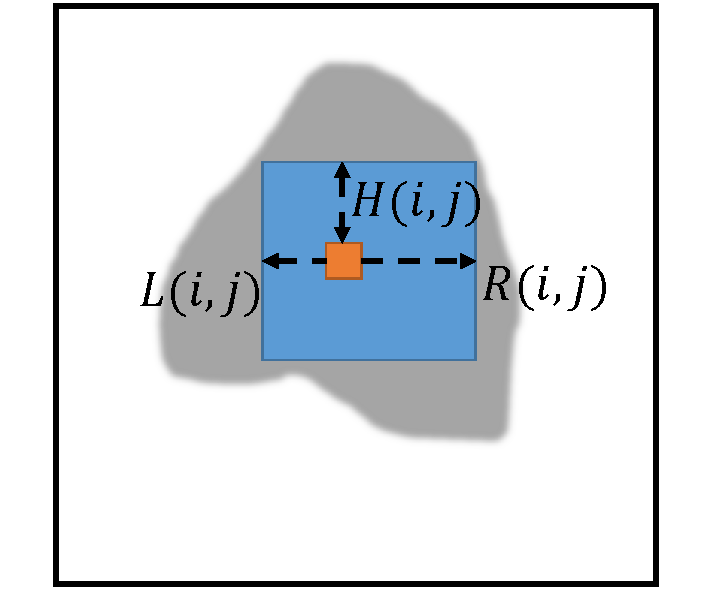
\includegraphics[width=8cm]{maximal_rectangle}
    \caption{The grey area denotes the all 1's area; the orange cube denotes $m[i][j]$; the blue rectangle denotes the largest rectangle in which $m[i][j]$ lies. $H(i,j)$ denotes the distance between the top of the rectangle and $m[i][j]$; $L(i,j)$ denotes the left index of the rectangle; $R(i,j)$ denotes the right index of the rectangle.}
    \label{fig:maximal_rectangle}
\end{figure}

Thus, the area $\bm{M}$ of the largest rectangle can be calculated as:
$$\bm{M}=\max_{i,j}\{H(i,j)(R(i,j)-L(i,j)+1)\}$$

\subsection{96. Unique Binary Search Trees}

\paragraph{Description}

Given n, how many structurally unique BST's (binary search trees) that store values 1...n?

For example,
Given n = 3, there are a total of 5 unique BST's.

\paragraph{Solution}
$$T(n)=\sum^{n-1}_{k=0}{T(k)T(n-k-1)}$$
$T(n)$ denotes the number of structurally unique BST's that store values $1,\cdots,n$. If we take $k+1$ as the root of the BST, then the left child has values $1,\cdots,k$ and the right child has values $k+2,\cdots,n$. Thus, the left child has $k$ values and the right one has $n-k-1$ values.

\subsection{72. Edit Distance}

\paragraph{Description}

Given two words word1 and word2, find the minimum number of steps required to convert word1 to word2. (each operation is counted as 1 step.)

You have the following 3 operations permitted on a word:
\begin{itemize}
    \item Insert a character
    \item Delete a character
    \item Replace a character
\end{itemize}

\paragraph{Solution}

\begin{equation*}
    T(i,j)=\begin{cases}
    T(i-1,j-1) & w_1[i]=w_2[j]\\
    \min\{T(i-1,j),T(i,j-1),T(i-1,j-1)\}+1 & w_1[i]\neq w_2[j]
    \end{cases}
\end{equation*}
$T(i,j)$ denotes the edit distance between $w_1[1,\cdots,i]$ and $w_2[1,\cdots,j]$. If $w_1[i]=w_2[j]$, $w_1[i]$ and $w_2[j]$ can be removed together. If $w_1[i]\neq w_2[j]$, there exit three ways to convert $w_1$ to $w_2$:
\begin{itemize}
    \item Remove $w_1[i]$ from $w_i$, then convert $w_1[1,\cdots,i-1]$ to $w_2[1,\cdots,j]$.
    \item Convert $w_1[1,\cdots,i]$ to $w_2[1,\cdots,j-1]$, then add $w_2[j]$.
    \item Convert $w_1[1,\cdots,i-1]$ to $w_2[1,\cdots,j-1]$, then replace $w_1[i]$ with $w_2[j]$.
\end{itemize}